\documentclass[a4paper,11pt]{article}
\pdfoutput=1 % if you are submitting a pdflatex (i.e. if you have
             % images in pdf, png or jpg format)

\usepackage{color}
\usepackage{jinstpub} % for details on the use of the package, please
                     % see the JINST-author-manual


\title{Investigation of Dark Matter Detection Capabilities in a Large Liquid Argon Time Projection Chamber}


%% %simple case: 2 authors, same institution
%% \author{A. Uthor}
%% \author{and A. Nother Author}
%% \affiliation{Institution,\\Address, Country}

% more complex case: 4 authors, 3 institutions, 2 footnotes
\author[a]{H. Back}
\author[a]{E. Church} %\note{Corresponding author.}}
\author[a]{C. Jackson}
\author[a]{R. Saldanha}


% The "\note" macro will give a warning: "Ignoring empty anchor..."
% you can safely ignore it.

\affiliation[a]{Pacific Northwest National Laboratory, Richland, WA 99354}

% e-mail addresses: only for the corresponding author
\emailAdd{eric.church@pnnl.gov}




\abstract{Liquid Argon Time Project Chambers (LArTPCS) are planned to comprise  the future of the U.S. High Energy Physics neutrino program. In particular, this detector technology will form the basis for the 40 kton DUNE experiment, beginning roughly in 2024. In this paper we focus on the dual phase far detector design and ask what changes to it may allow one of the four 10 kt modules to be sensitive to heavy WIMP dark matter detection. We show that with control over backgrounds and the use of argon depleted of $^{39}$Ar, which may be commercially available on that timescale, along with a significant increase in light detection, allows for a competitive WIMP detection sensitivity, particularly above 100 GeV.}



\keywords{Only keywords from JINST's keywords list please}


\arxivnumber{1234.56789} % only if you have one

\begin{document}
\maketitle
\flushbottom

\section{Introduction}
\label{sec:intro}

LArTPCs have been in use in neutrino physics in the ICARUS~\cite{ICARUS} experiment and most recently in the MicroBooNE detector~\cite{MicroB}. Two more LArTPC detectors are currently under construction on the Fermilab campus.

The culmination of the U.S. LArTPC program will be the construction of the 4-module 40 kt DUNE detector, to be located at the 4850 foot level of the Sanford Underground Research Facility near Lead, South Dakota. Data taking for the first two 10 kt modules -- one single liquid phase (SP), and the other dual phase (DP) -- is set to begin in 2024, though the full power neutrino beam is not scheduled to arrive until 2026. The third module is slated as either SP or DP and the exact technology for the fourth module is currently unspecified. This fourth 10 kt detector is known, therefore, as the module of opportunity. The main charge for investigators putting forward ideas for this module is that the main neutrino physics program of detection of the Charge Parity (CP) phase and the mass hierarchy determination are not compromised.

There are many suggested modifications under discussion currently within the collaboration which will take advantage of R\&D which are presumed to be available on the 2026 timescale. Few ideas for this module of opportunity to our knowledge, however, consider expanding or improving the non-neutrino beam physics program. 

We take note of the following  deficiencies in the DUNE program, as pointed out in the CDR~\cite{TDR} and in internal DUNE discussions. The Supernova explosion detection efficiency is lower than had been specified in the CDR (?), particularly at low energies; the solar neutrino program, recently being planned would benefit from a lower  threshold than the current ~10 MeV; formation of light "flashes" for determination of T0 in all manner of physics events is poor for low energy events, especially far from the light collectors. All of these problems have as their root causes  poor light collection and radioactive backgrounds in both the SP and DP detectors.

Explicitly, this paper proposes that  addressing these problems with sufficient seriousness provides a viable path to making the DUNE detector sensitive to detection of high mass dark matter. In this paper we discuss the possibility of a detector filled with 17 kt of argon depleted of $^{39}Ar$ that allows for an inner, radio-pure, self-shielded 1 kt volume of liquid argon.  We propose viewing that volume with light detection that can yield 100 photons/$keV$. We make three calculations that yield the conclusion that this detector can be a competitive DM detector on a schedule that expedites the world program, while preserving the main physics charge of DUNE.


\section {The LArTPC Far Detectors at DUNE}

The proposed DUNE Single Phase far detector is different from the preceding detectors in a few ways. First, it is comprised of modular blocks called Anode Plane Assemblies (APAs). One 10 kton cryostat is proposed to consist of ~125 (???) APAs. Each APA is comprised of one or two TPCs, which share a common high voltage cathode and two sets of three wire planes. A stainless steel cathode sits in the middle of any two APAs to provide the 500 $V/cm$ electric field for each TPC. A second key difference from existing LArTPCs is that light collection and wave-length shifting in the Single Phase DUNE far detectors resides in thin, so-called ARAPUCA assemblies that are mounted inside the wire anode planes.

The proposed DUNE Dual Phase far detector is, by contrast, one large, approximately 12x12x60 m$^3$ volume of liquid argon, without large panels of G10, stainless steel frames and wire assemblies in the liquid. The cryostat in which any 10 kton detector, SP or DP, is housed is the same. The drift is upward, across 12 meters of liquid argon. The design electric field is the same as for the SP detector. When ionization electrons arrive at the top liquid surface they are extracted with a high-field grid that produces an avalanche process, where at least a multiplication of ten (???) is achieved. Charge is collected onto positively biased pads, which are then read out to produce full x,y,z information (given a T0 constraint). 175 PMTs sit on the detector floor in the x-z plane and receive 2 photons/MeV to provide the needed T0 for an event.

\subsection{Proposed DUNE Dual Phase Design Modifications }
For our purposes, we propose using the DP design with its uninterrupted volume of liquid argon, free of radio-impure material in the bulk of the detector. We require the dual phase mechanism of charge extraction and multiplication.  However, we suggest to read out the photons, which are even more abundantly produced, after the multiplication stage rather than charge. Such a strategy allows to get to lower physics thresholds with high significance and simpler instrumentation than for charge readout. We propose that we use an inner 1 kT of argon of volume 6x6x20 m$^3$ for WIMP dark matter detection and more finely instrument S1 and S2 to read out that volume. Thus, for the S2 region we remove the charge readout pads in favor of either SiPMs or ARIADNE cameras~\cite{ARIADNE}. We point out that the latter camera is being developed in an intensive R\&D program with the express purpose of competing to serve as the DUNE DP S2 light readout, rather than S2 charge. ARIADNE appears to be able to easily provide the necessary spatial resolution for  multi-site nuclear recoil detection and at a fraction the cost needed for the same SiPM coverage. For S1 we propose to tile the bottom 8x22 m$^2$ with large $\cal{O}$(5cm$^2$) SiPMs.  The extra meter on all four sides allows for the multi-site rejection, which may be needed at low thresholds. If enough neutron moderator is used it may suffice to read out finely only over the 6x20 m$^2$.

A problem we know we will have to confront is which S1 light of the roughly twelve remaining $^{39}$Ar events in our depleted Argon goes with which S2 light. These ambiguities will be easier to resolve the better is our x-y position resolution.

\subsection{Detector Requirements for Dark Matter}
We require roughly 100 detected photons and the ability to achieve a 100 $keV$ threshold to detect dark matter in our inner 1 kton of fiducial argon. Net backgrounds of $\cal{O}(100)$ events from gammas and neutrons or lower are required. The energy threshold comes from the consideration of what is required to cover interesting parameter space for the WIMP search, though we also consider lower thresholds and lower backgrounds to show possible competitiveness with the world program. The 100 photons is a minimum requirement to be able to employ the technique widely-used in argon dark matter searches of pulse-shape discrimination (PSD). We will discuss this in a coming section at greater detail.

\subsubsection{DUNE Dual Phase Light Detection}
 We will want both $S1$ and $S2$, as in any dual phase dark matter detector. This added photon collection allows to detect $x,y,z$ from $S2$ and $S1$ combined information, while also contributing to the energy measurement that comes from $S1$.

\subsection{Relevant Backgrounds}
Neutrons enter from the walls from the Uranium/Thorium chain, as well as from detector materials and from Radon alpha,n reactions that may allow neutrons to mix into the argon itself. We will show that neutrons from walls can be ameliorated. Radon-induced neutrons will be dealt with in the cryogenic system.

For this potential new 10 kt module in DUNE we add 50 cm of poly inside the cryostat lining of the geometry of our model, informed by studies~\cite{beacom} that other solar neutrino measurements will require this neutron shielding, as well. This simple tactic reduces external neutron penetration effectively.

Next, gammas may enter from the outside materials and could conceivably penetrate into our fiducial inner 1 kt, despite self shielding. Here we will investigate the highest suspected radiological background gamma sources in DUNE and demonstrate that they are far sub-dominant to the relic $^{39}$Ar content of our underground argon, and thus taken care of by PSD.

\subsubsection{Gammas}
Gammas enter dominantly from $^{40}$K in the G10 in the detector materials. The DUNE background taskforce estimates these~\cite{bgd-taskforce} at 4.9 Bq/kg entering from the G10 circuit boards. We thus perform a study in which we run $^{40}$K decays from our detector ceiling where the G10 would be. We presume a 3mm thick 10mx58m sheet of G10; we find that the 1.46 MeV gammas appear at the sub $10^{-3}$ level per kt-year and ignore this background subsequently.

We also simulate $^{208}$Tl decays since that particular isotope is part of the Th/U decay chain, and the 2.61 MeV daughter gammas are less self-shielded than the lower energy $^{40}$K gammas. With simulations, using the DUNE background taskforce's 25 mBq/kg from G10, we find five [3] (7) [ events of 27E6 initial decays survive above 75 (100) [50] keV into our inner volume. This scales to 185 (110) [270] events per year. This is easily removed via PSD.


\subsubsection{Neutrons}
There are not only nuclear scatters from neutrons, but there are also n,Ar to Ca,$\gamma$ (neutron capture) reactions in the argon bulk. However, while indeed a 6-9 MeV capture $\gamma$ is a background to solar $\nu_e$ charged current reactions, it will not be confused for a WIMP scatter. Thus, while neutron amelioration benefits will accrue to any DUNE solar neutrino program, we concern ourselves in this paper with reducing and removing neutron nuclear scatters.

\subsubsection{Radon}
Radon swirls around in the bulk of the detector, and its $\alpha$ decays interact on argon neutrons, leading to neutrons that can mimic WIMP scatters.

We plan to use charcoal filters to control this background. 
RICHARD/CHRIS: please finish.

\subsection{Underground Argon}
Underground Argon has been employed for Darkside50~\cite{darkside50} which used argon depleted in $^{39}Ar$ by a factor of 1400 from its abundance in surface argon. Darkside20k plans to use this same source of argon.

HENNING/CHRIS/RICHARD more words here.... concluding with ...

Pulse Shape Discrimination (PSD) allows a nuclear recoil to electron rejection of $10^{-9}$ in Darkside50.

A benefit of employing depleted argon, apart from making DUNE potentially able to do dark matter physics, is that the mere reduction of the $^{39}$Ar background activity allows for far superior matching of detected light and charge activity, particularly for the sub-10 $MeV$ range than is currently achievable (see Figure~\ref{fig:flashmatch}). Strong model dependence is involved in statements about detection efficiency for extra-galactic SN explosions, but we can confidently state that galactic SNE detection below 12 MeV should increase from the current \_\_\_.

\begin{figure}[t]
\begin{centering}
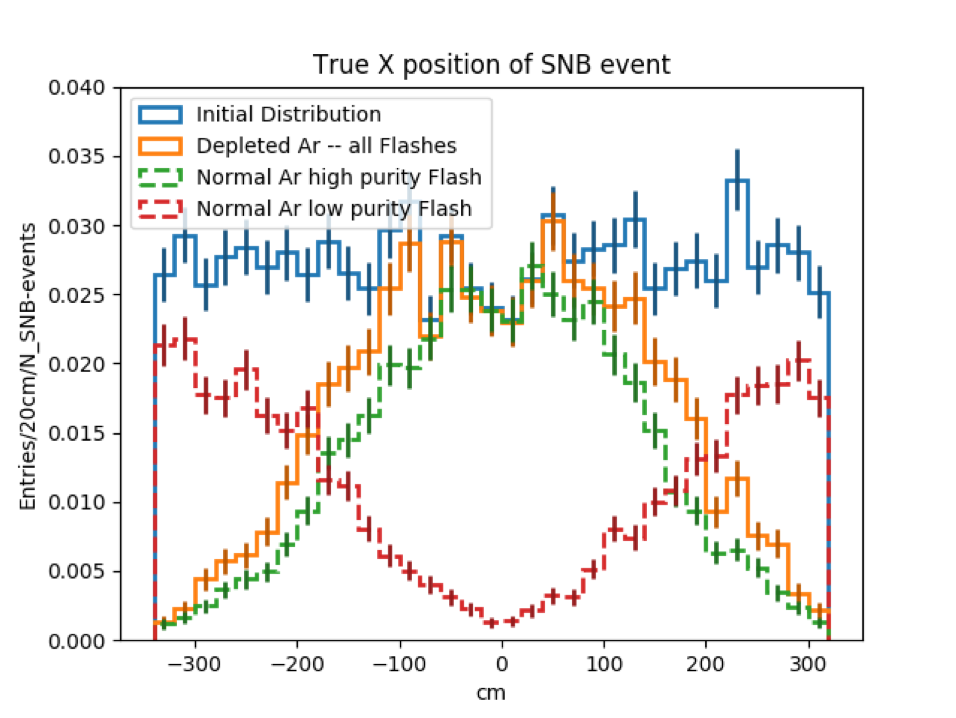
\includegraphics[width=0.90\columnwidth]{Figures/flashmatch.png}
\par\end{centering}

\caption{Shown is the improved optical "flash" match to charge activity with reduced $^{39}$Ar. At large values of the drift dimension, well away from the single phase light detectors, the optical "flash" is far more liable to be correctly identified with  the supernova event's drifted charge and not plagued by low purity mis-identification as in the red with normal argon. Certainly, better light detection as proposed here increases the match efficiency.  \label{fig:flashmatch}}
\end{figure}

We note that with the expected 10$^{-5}$ depletion factor, ~12 flashes from $^{39}Ar$ events remain in the drift volume which must be rejected by the S1 and S2 systems. This is an offline task and benefits from particularly fine $x-y$ position resolution, though we don't demonstrate the needed requirement here.



\section{Calculations}
\subsection{Neutron Amelioration}

Upon running various gamma and neutron simulations and using information from the DUNE background taskforce, we find that the biggest background source in our chosen detector configuration is from external neutrons emanating from the cavern walls in the Uranium/Thorium chain.
While there are great uncertainties on the {n,Ar} reaction, we take a worst case scenario, as is in fact coded into Geant4 10.5 that neutrons proceed mostly transparently through argon. We know there are results~\cite{svoboda} in process that will only increase this cross-section. We ameliorate the neutron problem in two ways: with a proposed 50 cm plastic liner just inside the cryostat and with a reconstruction technique that allows to detect and remove multi-site neutron-induced nuclear recoil events.

See figure~\ref{fig:neutrons} for the incident DUNE neutron spectrum (graph-clicked from~\cite{bgd-taskforce}) and the neutron background which survives propagation and multi-site rejection in the inner 1 kt.

\begin{figure}[t]
\begin{centering}
%%\includegraphics[width=0.90\columnwidth]{Figures/NeutronKE_interact005_25_dunedistn.png}
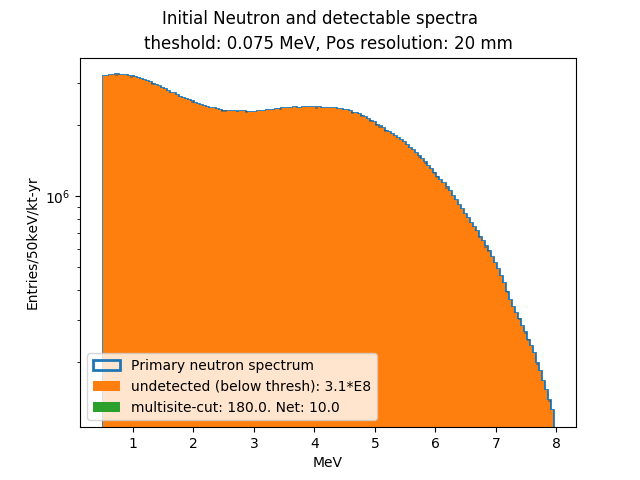
\includegraphics[width=0.90\columnwidth]{Figures/NeutronKE_interact0075_20_dunedistn_25cmPoly.png}
\par\end{centering}

\caption{ Shown are the external neutron spectrum emanating from outside the cryostat at an assumed 10 Hz and the surviving events in the inner 1 kt, and the net remaining contribution after multi-site cuts are applied. We presume a 75 keV n.r. detection threshold here and a 20mm or greater multi-site minimal detectable distance. This simulation uses a 25 cm Poly liner in the cryostat.
\label{fig:neutrons}}
\end{figure}

\subsection{Photon Counting}
CHRIS J's toy simulation. 
Reproduces the DP default 2 ph/MeV.
What is necessary is to get a plausible 1 ph/keV.

DUNE DP's OPTICAL SIM. Can we check that we corroborate anything done already? Please state even if qualitatively the need for wls foils, etc, and if they may need to be in the bulk argon. I've said something to this effect in the conclusion.

\subsection{Pulse Shape Discrimination}
Richard's Darkside-based simulation that shows 100 photons at 100 keV can allow an argon gamma background at the level of the neutron background of ~50 evts. We show an $^{39}$Ar beta/n rejection factor here of $10^{-9}$ at 100 keV and even at 75 keV.

RICHARD will check these words and that he's done this correctly.

\section{Sensitivity for Dark Matter Detection}

We use the standard WIMP code~\cite{loer-code} that takes into account all the complications of WIMP scattering off heavy target nuclei, including seasonal variation and standard structure function uncertainties. In figure~\ref{fig:Sensitivity} we show three world-leading, experimental heavy noble limits. We also show the 90\% sensitivity reach of the liquid argon  Darkside20k~\cite{darkside20k} experiment, along with that of the full GADMC limit~\cite{gadmc}, which is the planned follow-on to Darkside20k. We point out that GADMC is built to get below the neutrino floor. We overlay three potential sensitivities from the DUNE 4$^{th}$ detector in which we imagine running our 1 kt fiducial volume for 3 years. Such a strategy would produce a physics result on the timescale of the Darkside20k result and ahead of the would-be GADMC result.


\begin{figure}[t]
\begin{centering}
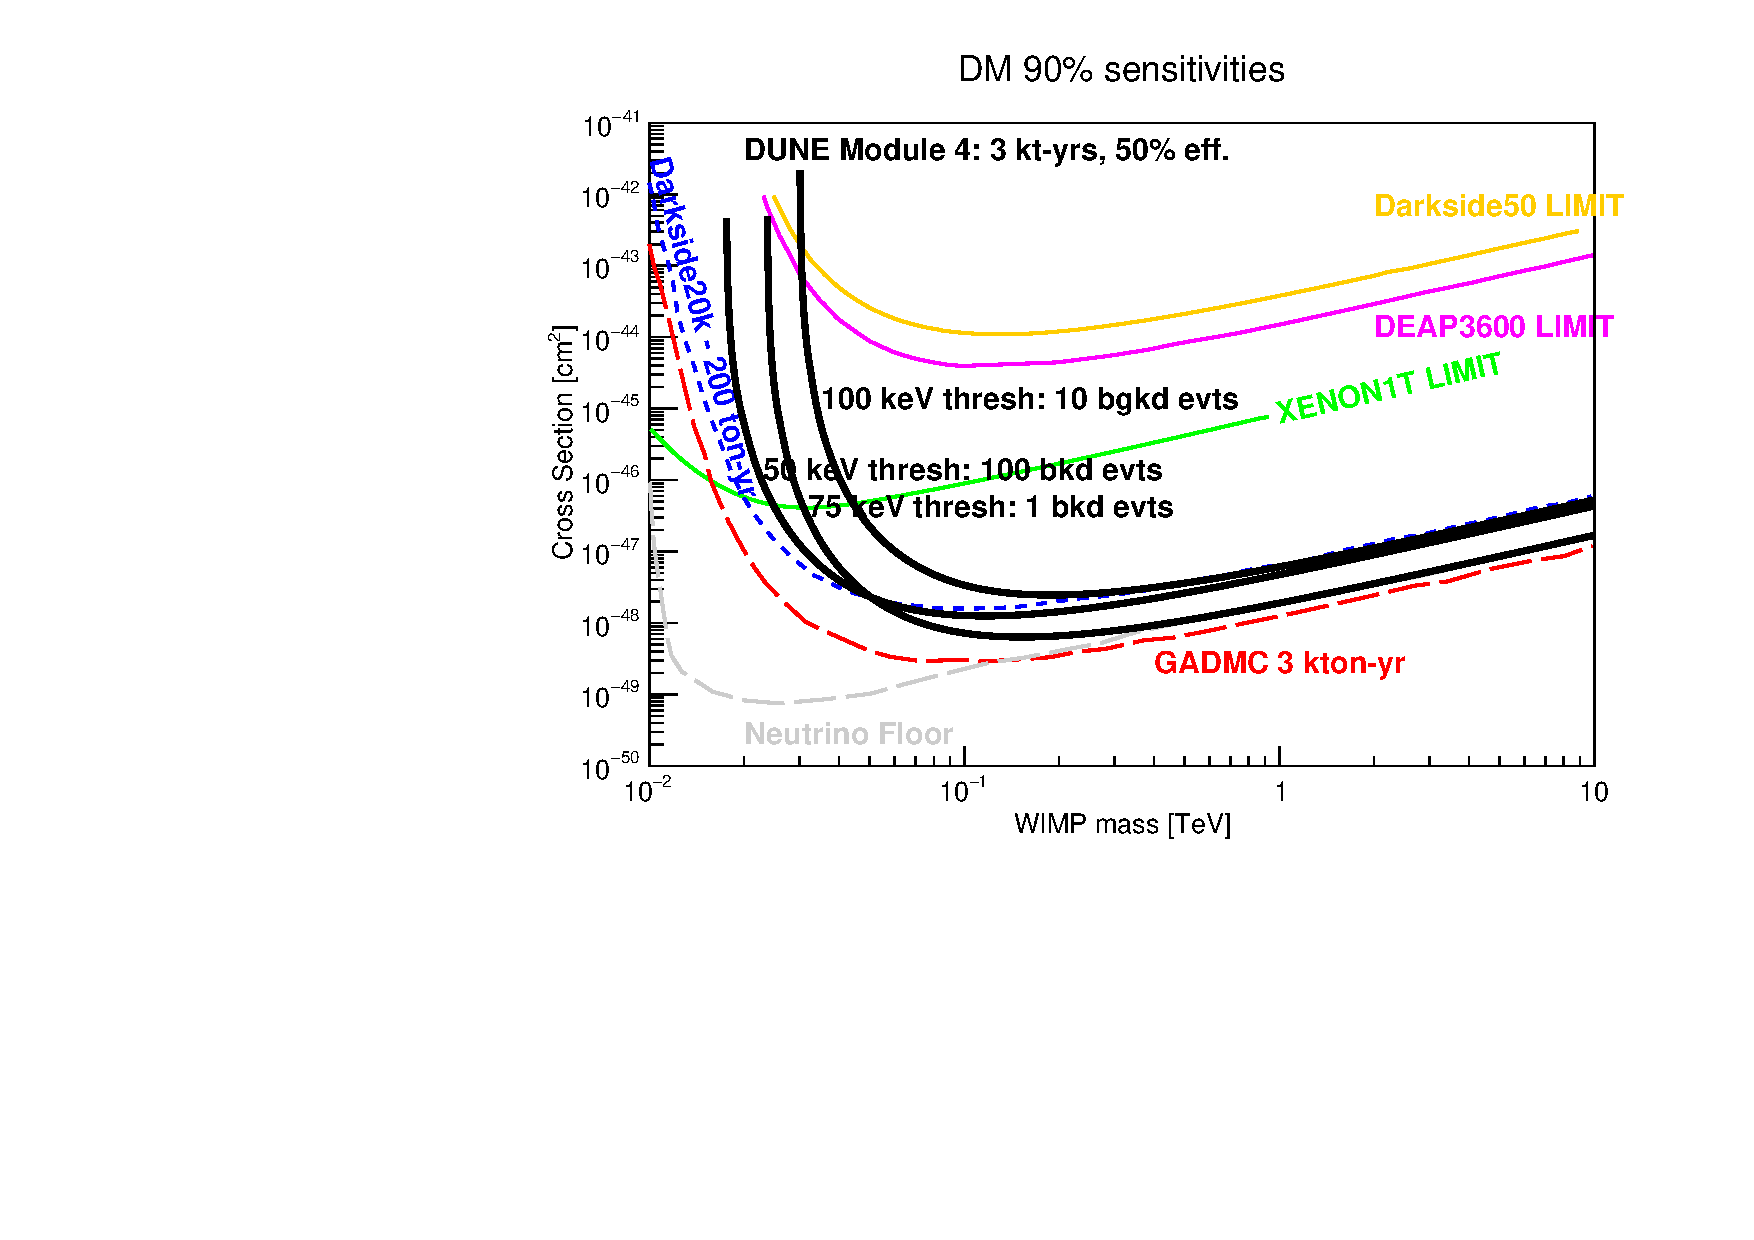
\includegraphics[width=0.90\columnwidth]{Figures/paper_placeholder.pdf}
\par\end{centering}

\caption{Shown are the achieved 90\% limits in solid colored lines for various experiments for WIMP Dark Matter. Dashed lines for proposed argon experiments are overlaid. Three DUNE possibilities for module 4 for various thresholds and expected backgrounds, as discussed in the text, are shown in black lines. \label{fig:Sensitivity}}
\end{figure}

\section{Results and Discussion}

Table~\ref{table:DUNE} shows estimated backgrounds for one would-be DUNE dark matter scenario that we investigate. The scenarios vary by energy threshold and assumed background, from likely achievable to extremely ambitious. 


\begin{table}[h]
\begin{tabular}{ l c c r}
%%%%\multicolumn{4}{c}{\bf Background in 10 kt-yr 100 keV for threshold, (25 cm) 50cm thick Poly cryostat liner} \\
 Radioactive particle & Emanation source & Amelioration strategy & counts/kt-yr (before PSD)\\
\hline
 neutrons  & external rock & Poly lining, multi-site rejection & $< 1$ (10)\\
  $^{40}$K gammas &  G10 & Self-shielding & $< 10^{-3}$ \\
$^{208}$Tl gammas & $^{232}$Th chain in G10 & Self-shielding & 185\\
 $^{39}$Ar betas & bulk argon & Using depleted argon and PSD & 0.23  \\
\end{tabular}
\label{table:DUNE}
\caption{Backgrounds considered and count rates per year in inner 1 kt fiducial volume. Presumes $^{39}$Ar depleted at $10^{-5}$, a multi-site rejection with 20cm resolution and a 100 keV nuclear recoil detectable threshold. Results are for a 50cm thick Poly cryostat lining, though we show for neutrons in parenthesis the number for a 25cm lining. Gamma backgrounds are shown before application of PSD, which reduces them by $10^{-9}$ and thus renders them irrelevant.}
\end{table}

We see from figure~\ref{fig:Sensitivity} that the dedicated liquid argon Dark Matter detectors have an advantage below the 10-30 GeV WIMP mass range over anything DUNE can likely do. One imagines that a 50 keV threshold for a DUNE 4$^{th}$ detector module will be very difficult to achieve, given the sheer size of the detector and industrial materials that must be employed. We believe a 100 keV threshold is achievable with some reasonable radiopurity controls. Further, we have some confidence based on our own toy Monte Carlo and~\cite{privateconv:flavio} that 100 photons at 100 keV can be achieved with upgraded dense optical coverage, as we suggest here. The resulting two sensitivity curves show an interesting coverage with respect to Darkside20k. Further, we show that an ambitious background reduction and an intermediate threshold to the two just mentioned, in fact, allow to get to the neutrino floor in a manner akin to GADMC's plans.

We remind that at least one further problem must be overcome: at the claimed level of rejection of spurious $^{39}$Ar activity, there remains on the order of twelve decays during the vertical drift time in our DP detector which must be distinguished from each other and rejected. We presume this is a relatively straightforward offline task that with sufficiently light detector granularity can be tackled successfully.

\section{Conclusion}
We show in this study that a large LArTPC detector filled with argon depleted at the level of $10^{-5}$ of $^{39}$Ar can be a world-competitor for high mass WIMP detection, given improved light detection for a self-shielded inner 1 kt of liquid  inside a DUNE-like 10 kt detector. We have some  confidence that commercial sources of such underground argon are obtainable on the DUNE 4$^{th}$ detector -- the so-called module of opportunity -- timescale of the mid-to-late 2020's. This allows the use of the widely understood technique employable in argon of pulse shape discrimination (PSD) to markedly suppress gamma backgrounds. 

We show with a toy monte carlo that this much-improved light detection over the current DUNE dual phase design may likely be achieved. A denser array of photosensors, ala some combination of SiPMs and the ARIADNE camera, are required compared to the current DUNE DP design, as are reflective foils potentially placed in the argon. We show that neutrons in our inner 1 kt may be removed with a modest Poly lining in the cryostat. PSD may be employed to remove remaining $e-/\gamma$ background. Further, very aggressive radio-purity controls might allow a slight lowering of the threshold and background and, thus, the ability to get to the neutrino floor.

With a detector module such as the one described here, a broad low-energy physics program for DUNE would be enabled that does not perturb the main neutrino program. Efficient measurements of solar neutrinos and supernovae reactions, at the least, become enabled in such a detector. In fact, we remark that this module, with its low energy threshold for the inner fiducialized volume, could serve as the supernova event trigger for the full 40 kt DUNE far detector complex.


% We suggest to always provide author, title and journal data:
% in short all the information that clearly identify a document.

\begin{thebibliography}{99}

\bibitem{ICARUS}
The ICARUS Collaboration, \emph{Design, construction and Tests of the Icarus T600 Detector}, NIMA {\bf 55}, Issue 3, (2004) p329.
\bibitem{MicroB}
The MicroBooNE Collaboration, \emph{Design and Construction of the MicroBooNE Detector}, JINST {\bf 12} (2017) p2017.
\bibitem{TDR}
{\bf FIXME}
The DUNE Collaboration, \emph{The DUNE Far Detector Interim Design Report, Volume 1: Single Phase Module}, arXiv:1807.10327, 2018.

\bibitem{ARIADNE}
A. Roberts, P. Svihra, A. Al-Refaie, H. Graafsma, J. Küpper, K. Majumdar, K. Mavrokoridis, A. Nomerotski, D. Pennicard, B. Philippou, S. Trippel, C. Touramanis, J. Vann, \emph{First Demonstration of 3D Optical Readout of a TPC using a single photon sensitive Timepix3 based camera}, arXiv:1810.09955, 2018.

\bibitem{beacom}
Francesco Capozzi, Shirley Weishi Li, Guanying Zhu, John F. Beacom, \emph{DUNE as the Next Generation Solar Neutrino Experiment}, Phys. Rev. Lett. {\bf 123}, (2019) 131803.

\bibitem{darkside50}
The Darkside Collaboration, {\emph Results from the first use of low radioactivity argon in a dark matter search} Physical Review D, 93 (2016) p081101.

\bibitem{svoboda}
R. Svoboda, {\emph Neutrons in DUNE},
https://agenda.ciemat.es/event/1127/contributions/2225/attachments/1693/2076/20191121\_DUNE\_Neutrons.pdf, CIEMAT Conference, Madrid, Spain (2019).

\bibitem{bgd-taskforce}
Rechenmacher, Stock, Haiston \emph{Radiological Background Model for DUNE MCCs},
https://indico.fnal.gov/event/17817/session/6/contribution/12/material/slides/0.pdf.

\bibitem{loer-code}
{\bf FIXME}
Loer+ Others???, \emph{Title}, \emph{J. Abbrev.} {\bf vol} (year) pg.

\bibitem{darkside20k}
The Darkside20k Collaboration, \emph{DarkSide-20k: A 20 Tonne Two-Phase LAr TPC for Direct Dark Matter Detection at LNGS},
 arXiv:1707.08145 (2017).

\bibitem{gadmc}
{\bf FIXME: NEED a CITATION<}
The GADMC Collaboration,  \emph{DarkSide-20k: A 20 Tonne Two-Phase LAr TPC for Direct Dark Matter Detection at LNGS},
 arXiv:1707.08145 (2017).

\bibitem{privateconv:flavio}
Flavio Cavana conversation, \emph{DUNE Module of Opportunity Workshop}, Brookhaven National Laboratory, November, 2019.


% Please avoid comments such as "For a review'', "For some examples",
% "and references therein" or move them in the text. In general,
% please leave only references in the bibliography and move all
% accessory text in footnotes.

% Also, please have only one work for each \bibitem.


\end{thebibliography}
\end{document}
